\AtBeginSection[]{
    \begin{frame}
        \frametitle{}
        \tableofcontents[currentsection]
    \end{frame}
}

%%%%%%%%%%%%%%%%%%%%%%%%%%%%%%%%%%%%

\section{AOMEA approach}

\subsection{Overview}

\begin{frame}{AOMEA approach}{Overview}

    \begin{figure}[h!]
        \centering
        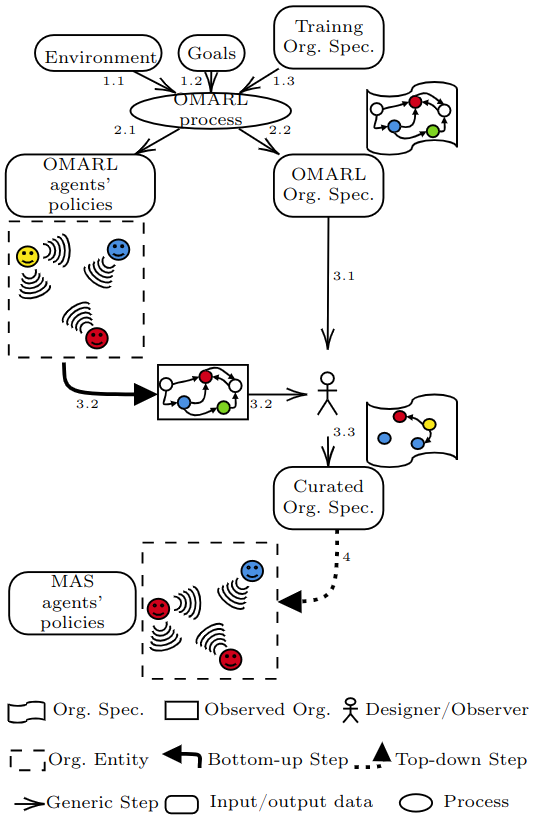
\includegraphics[width=0.3\linewidth]{figures/AOMEA_illustrative_view}
        \caption{A summary view of our approach to MAS design}
        \label{fig:design_approach}
    \end{figure}

\end{frame}


\begin{frame}{AOMEA approach}{Overview}

    \begin{columns}

        \begin{column}{0.5\textwidth}

            \textbf{Phase 1: Modeling}

            \begin{itemize}
                \item Designers have to manually develop a simulation of the target environment ($1.1$) where agents must cooperate to achieve the designer's goal efficiently ($1.2$);
                \item Designers can link parts of an agent's history with known OS;
                \item Optionally, designers may also want to integrate constraints as well ($1.3$).
            \end{itemize}

        \end{column}

        \begin{column}{0.5\textwidth}
            \centering
            \adjustbox{trim={0.\width} {0.82\height} {0.\width} {0.\height}, clip}{%
                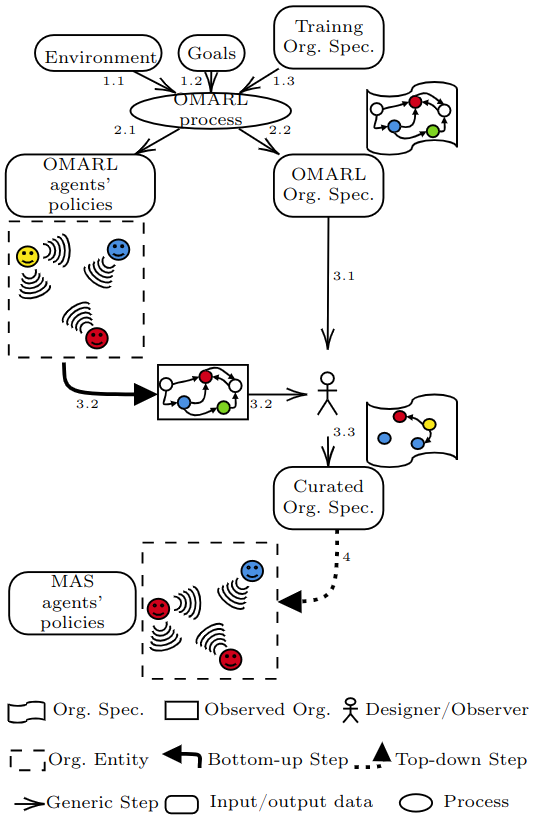
\includegraphics[width=\linewidth]{figures/AOMEA_illustrative_view}
            }
        \end{column}

    \end{columns}

\end{frame}

\begin{frame}{AOMEA approach}{Overview}

    \begin{columns}

        \begin{column}{0.5\textwidth}

            \textbf{Phase 2: Solving}

            \begin{itemize}
                \item a MARL algorithm is used and satisfy constraints on policies regarding known relations between histories and OS;
                \item finds optimal policies satisfying the given design organizational specifications ($2.1$);
                \item gets the associated OS ($2.2$)
            \end{itemize}

        \end{column}

        \begin{column}{0.5\textwidth}
            \centering
            \adjustbox{trim={0.\width} {0.56\height} {0.\width} {0.\height}, clip}{%
                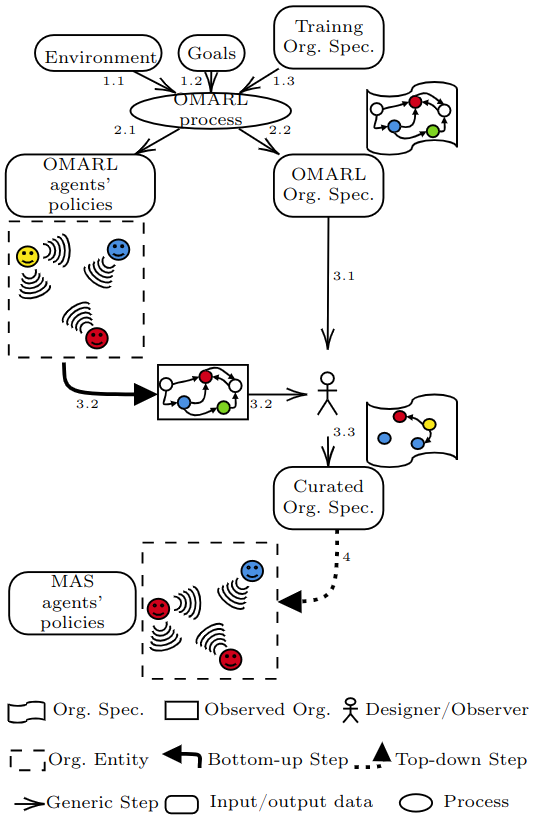
\includegraphics[width=\linewidth]{figures/AOMEA_illustrative_view}
            }
        \end{column}

    \end{columns}


\end{frame}

\begin{frame}{AOMEA approach}{Overview}

    \begin{columns}

        \begin{column}{0.5\textwidth}

            \textbf{Phase 3: Analyzing}

            \begin{itemize}
                \item Designers observe the trained agents' policies ($3.2$);
                \item Designers takes into account the inferred associated OS ($3.1$) to understand they reach the goal;
                \item Designers get some indications of the OS capable of achieving the goal: the curated OS ($3.3$).
            \end{itemize}


        \end{column}

        \begin{column}{0.5\textwidth}
            \centering
            \adjustbox{trim={0.\width} {0.35\height} {0.\width} {0.188\height}, clip}{%
                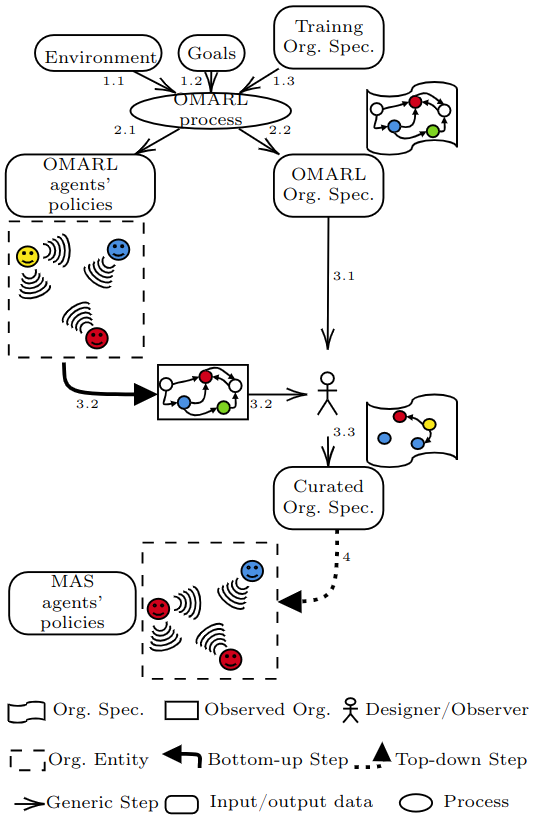
\includegraphics[width=\linewidth]{figures/AOMEA_illustrative_view}
            }
        \end{column}

    \end{columns}

\end{frame}

\begin{frame}{AOMEA approach}{Overview}

    \begin{columns}

        \begin{column}{0.5\textwidth}

            \textbf{Phase 4: Developing}

            \begin{itemize}
                \item Designers takes into account the curated organizational specifications as a blueprint for implementing a MAS;
                \item Regular MAS development with one of the available methods can be applied hence addressing safety issues;
                \item Implemented agents are launched in simulations for final assessing.
            \end{itemize}

        \end{column}

        \begin{column}{0.5\textwidth}
            \centering
            \adjustbox{trim={0.\width} {0.15\height} {0.\width} {0.57\height}, clip}{%
                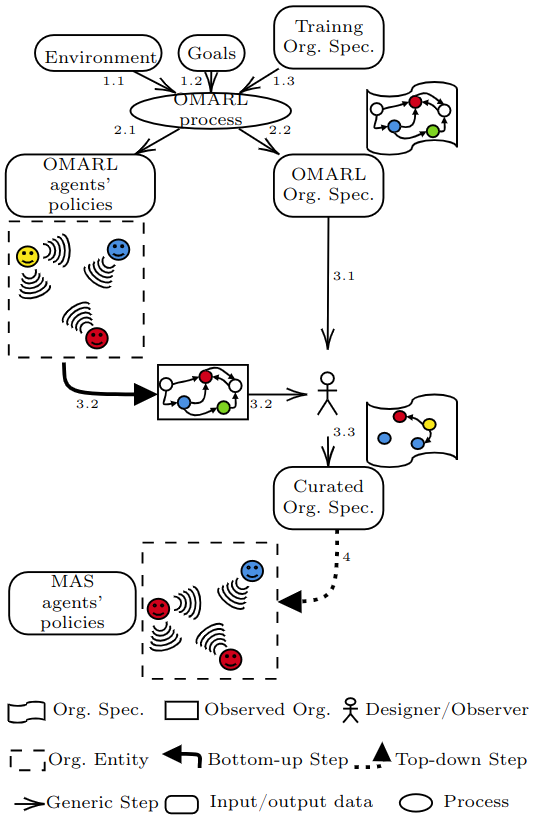
\includegraphics[width=\linewidth]{figures/AOMEA_illustrative_view}
            }
        \end{column}

    \end{columns}

\end{frame}


\subsection{Theoretical core}

\begin{frame}[allowframebreaks]{AOMEA approach}{Theoretical core}

    \begin{block}{\emph{Partial Relations with Agent History and Organization Model} algorithm (PRAHOM)}
        Synthesis of two processes that fall into the OMARL purposes
        \begin{enumerate}
            \item \textbf{Inferring Organizational Specifications}: gets the specifications from the agents' policies;
            \item \textbf{Constraining Policies Space}: gets the joint-policies satisfying the given design specifications
        \end{enumerate}
    \end{block}
\end{frame}

\begin{frame}{AOMEA approach}{Theoretical core}

    \textbf{Inferring Organizational Specifications}

    \begin{columns}

        \begin{column}{0.3\textwidth}

            \begin{itemize}
                \item \textbf{Knowledge-based Organizational Specifications Identification (KOSIA)}
                \item \textbf{General Organizational Specifications Infererence (GOSIA)}
            \end{itemize}

        \end{column}

        \begin{column}{0.8\textwidth}
            \begin{figure}
                \centering
                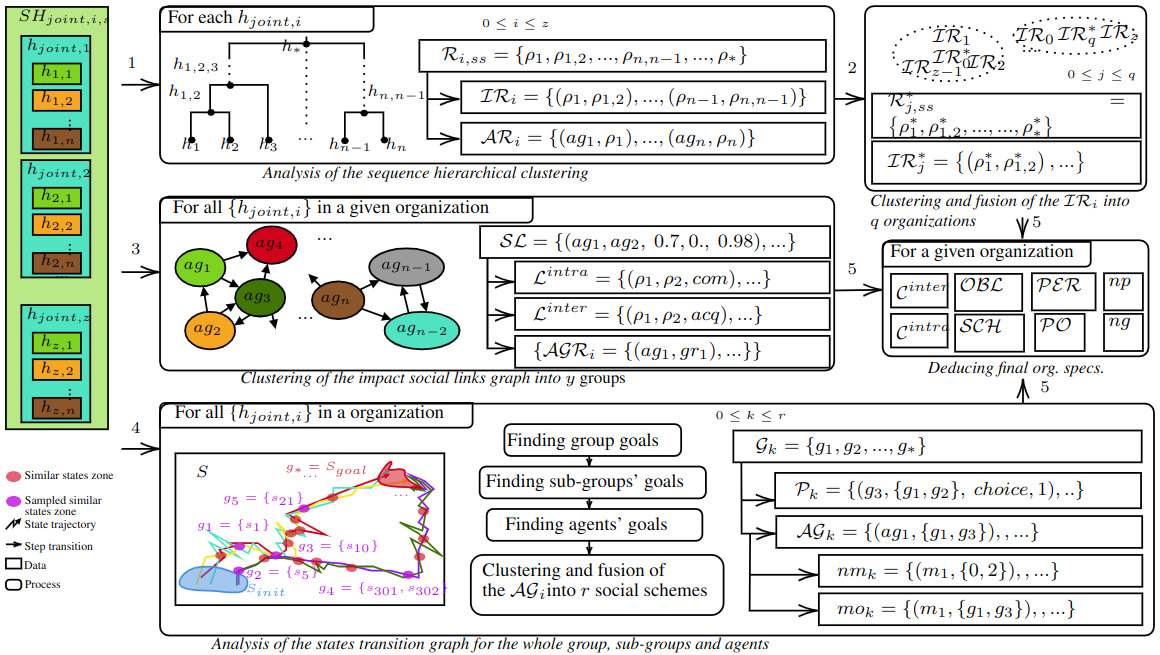
\includegraphics[width=0.95\linewidth]{figures/GOSIA_view.png}
                \caption{A summary view of the GOSIA process}
                \label{fig:gosia_process}
            \end{figure}
        \end{column}

    \end{columns}





\end{frame}

\begin{frame}{AOMEA approach}{Theoretical core}

    \textbf{Constraining Policies Space} during training

    \begin{columns}

        \begin{column}{0.3\textwidth}

            \begin{itemize}
                \item At each step, available actions set is changed to match policy constraints defined by users;
                \item Constraints integrated through: external correction, learning, internal policy change.
            \end{itemize}

        \end{column}

        \begin{column}{0.8\textwidth}
            \begin{figure}
                \centering
                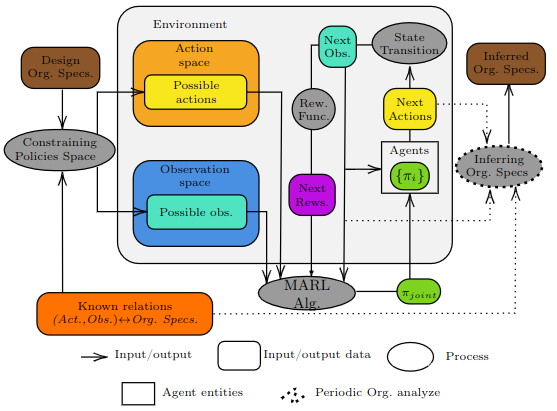
\includegraphics[width=0.7\linewidth]{figures/prahom_view.png}
                \caption{A summary view of the PRAHOM process}
                \label{fig:prahom_process}
            \end{figure}
        \end{column}

    \end{columns}

\end{frame}

\subsection{Engineering tool}

\begin{frame}[fragile]{AOMEA approach}{Engineering tool}

    \begin{block}{\emph{PRAHOM PettingZoo Wrapper}\label{PettingZoo-wrapper}}
        \begin{itemize}
            \item Uses \textbf{PettingZoo}: a library with a standardized API that facilitates the application of MARL algorithms;
            \item Proposed as a tool to help automate the setting up of \emph{PRAHOM} for a given PettingZoo environment
        \end{itemize}
    \end{block}

    \

    \begin{lstlisting}[language=Python, caption=PRAHOM PettingZoo Wrapper basic use, label={lst:wrapper_basic_use}]
    from omarl_experiments import prahom_wrapper
    env=PettingZoo_env.parallel_env(render_mode="human")
    specs_to_hist={"structural_specifications":{"roles":{"follower":{"23":41,"14":[74,0]}}...},"functional_specifications":{"links":{"(leader,follower,aut)":".*14.*?89"}...}...}
    policy_specs_constr={"agent_0":{"structural_specifications":"roles":["follower"]}}
    env=prahom_wrapper(env,action_to_specs,training_specs)
    env.train("default_PPO")
    trained_specs,agent_to_specs=env.prahom_specs()
    \end{lstlisting}

\end{frame}
